% !TeX spellcheck = cs_CZ
%{\tikzset{external/prefix={tikz/FYZII/}}
% \tikzset{external/figure name/.add={ch14_}{}}
%---------------------------------------------------------------------------------------------------
% file fey2ch14.tex
%---------------------------------------------------------------------------------------------------
%====================Kapitola: Magnetické pole v různých případech =================================
\setchaptertoc
\chapter{Magnetické pole v různých případech}\label{fyz:IIchapXIV}


  \section{Vektorový potenciál}\label{fyz:IIchapXIVsecI}
  \section{Vektorový potenciál daných proudů}\label{fyz:IIchapXIVsecII}
  \section{Přímý vodič}\label{fyz:IIchapXIVsecIII}
  \section{Dlouhý solenoid}\label{fyz:IIchapXIVsecIV}
  \section{Pole malé smyčky. Magnetický dipól}\label{fyz:IIchapXIVsecV}
  \section{Vektorový potenciál obvodu}\label{fyz:IIchapXIVsecVI}
  \section{Biot-Savartův zákon}\label{fyz:IIchapXIVsecVII}

    \begin{figure}[ht!] %\ref{fyz:fig0673}
      \centering
      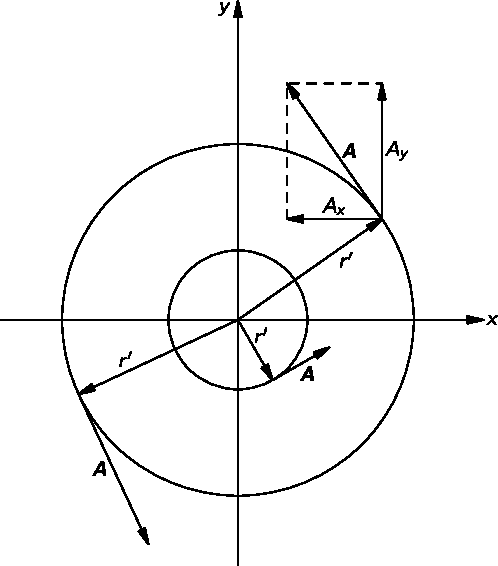
\includegraphics[width=0.7\linewidth]{fyz_fig0673.pdf}
      \caption{
               (\cite[s.~707]{Feynman02})}
      \label{fyz:fig0673}
    \end{figure}

    \begin{figure}[ht!] %\ref{fyz:fig0674}
      \centering
      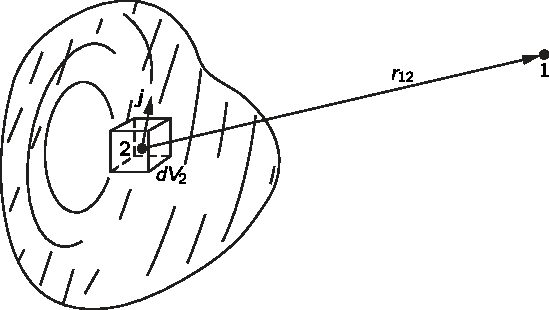
\includegraphics[width=0.7\linewidth]{fyz_fig0674.pdf}
      \caption{
               (\cite[s.~707]{Feynman02})}
      \label{fyz:fig0674}
    \end{figure}

    \begin{figure}[ht!] %\ref{fyz:fig0675}
      \centering
      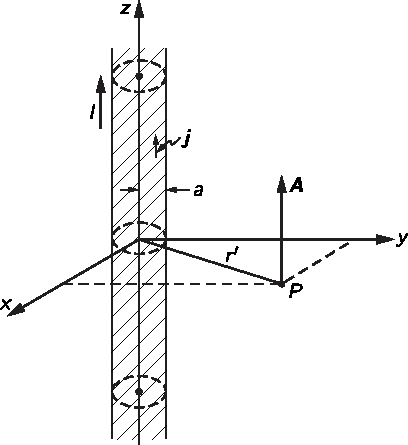
\includegraphics[width=0.7\linewidth]{fyz_fig0675.pdf}
      \caption{
               (\cite[s.~707]{Feynman02})}
      \label{fyz:fig0675}
    \end{figure}

    \begin{figure}[ht!] %\ref{fyz:fig0676}
      \centering
      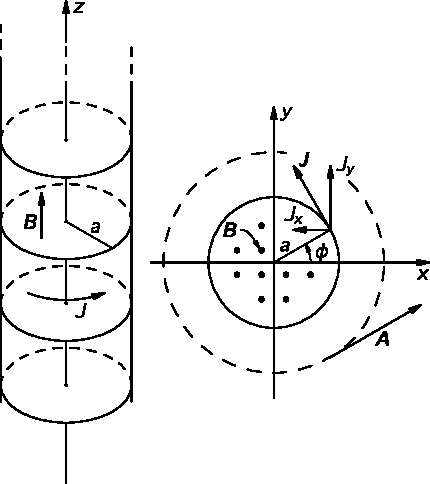
\includegraphics[width=0.7\linewidth]{fyz_fig0676.pdf}
      \caption{
               (\cite[s.~707]{Feynman02})}
      \label{fyz:fig0676}
    \end{figure}
    
    \begin{figure}[ht!] %\ref{fyz:fig0677}
      \centering
      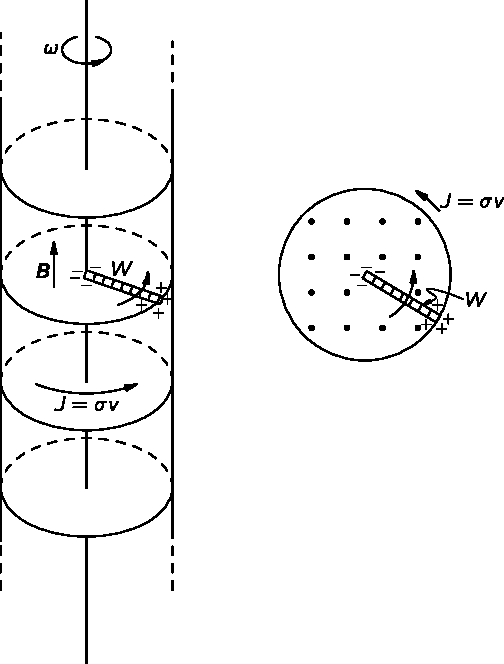
\includegraphics[width=0.7\linewidth]{fyz_fig0677.pdf}
      \caption{
               (\cite[s.~707]{Feynman02})}
      \label{fyz:fig0677}
    \end{figure}

    \begin{figure}[ht!] %\ref{fyz:fig0678}
      \centering
      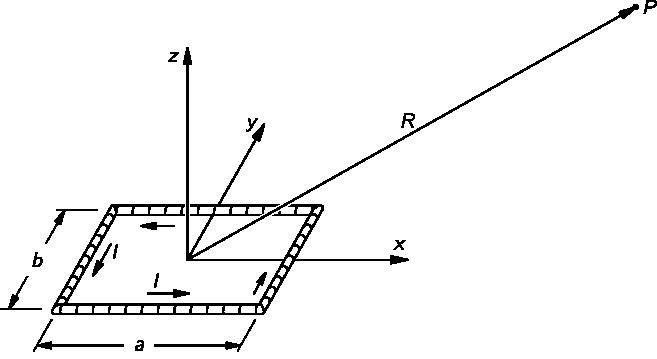
\includegraphics[width=0.7\linewidth]{fyz_fig0678.pdf}
      \caption{
               (\cite[s.~707]{Feynman02})}
      \label{fyz:fig0678}
    \end{figure}

    \begin{figure}[ht!] %\ref{fyz:fig0679}
      \centering
      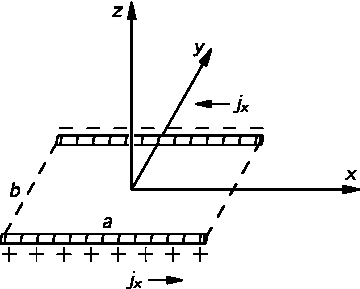
\includegraphics[width=0.7\linewidth]{fyz_fig0679.pdf}
      \caption{
               (\cite[s.~707]{Feynman02})}
      \label{fyz:fig0679}
    \end{figure}

    \begin{figure}[ht!] %\ref{fyz:fig0680}
      \centering
      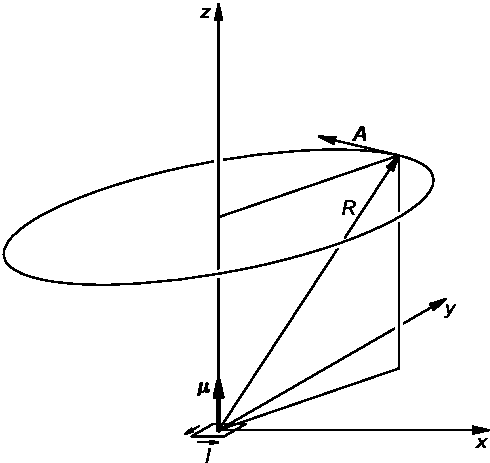
\includegraphics[width=0.7\linewidth]{fyz_fig0680.pdf}
      \caption{
               (\cite[s.~707]{Feynman02})}
      \label{fyz:fig0680}
    \end{figure}

    \begin{figure}[ht!] %\ref{fyz:fig0681}
      \centering
      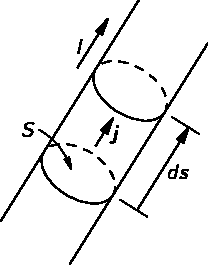
\includegraphics[width=0.5\linewidth]{fyz_fig0681.pdf}
      \caption{
               (\cite[s.~707]{Feynman02})}
      \label{fyz:fig0681}
    \end{figure}

    \begin{figure}[ht!] %\ref{fyz:fig0682}
      \centering
      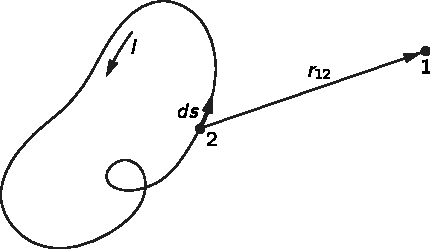
\includegraphics[width=0.7\linewidth]{fyz_fig0682.pdf}
      \caption{
               (\cite[s.~707]{Feynman02})}
      \label{fyz:fig0682}
    \end{figure}


    \todo[inline]{Kapitola fey2ch14 je nedodělaná, obsahuje pouze obrázky}
%} %tikzset
%~~~~~~~~~~~~~~~~~~~~~~~~~~~~~~~~~~~~~~~~~~~~~~~~~~~~~~~~~~~~~~~~~~~~~~~~~~~~~~~~~~~~~~~~~~~~~~~~~~
